\documentclass[runningheads]{llncs}

\author{
    Sokolov, B. \inst{1} \orcidID{0000-0002-2295-7570} \and
    Zakharov, V.\inst{1} \orcidID{0000-0002-2086-2041} \and
    Murashov, D.\inst{1} \orcidID{0000-0003-3163-3145} \and
    Murashova, M.\inst{2} \orcidID{0000-0002-9857-4779}
}

\authorrunning{B. Sokolov et al.}
\institute{St. Petersburg Institute for Informatics and Automation of the Russian Academy of Sciences \email{spiiran@iias.spb.su} \url{www.spiiras.nw.ru} \and Saint Petersburg State University of Aerospace Instrumentation (SUAI) \email{int@aanet.ru} \url{www.suai.ru}}

\title{An approach to fusing strategic objectives into agent-level decision making in load balancing}
\usepackage[T1]{fontenc}
\usepackage[colorinlistoftodos]{todonotes}
\usepackage{graphicx}
\usepackage{mathtools}
\usepackage{times}
\usepackage{kpfonts}
\usepackage{subcaption}
\usepackage{multirow}
\usepackage{tabularx}
\usepackage{array}
\usepackage{algorithm}
\usepackage{algpseudocode}
\usepackage{tabularx}

\graphicspath{{./img/}}

% Naming conventions
% <fn><m|l><NAME>
% fn - prefix to distinguish newly-defined commands. Stands for "function"
% m - stands for "math". Indicates that it is used in the context of a $math expression$.
% l - stands for "listing"

% Alternatives (nodes)
\newcommand{\fnmalts}{V_{N,1}, V_{N,2},\ldots}

% Aspects (nodes)
% arg 1 - indentifier of the level the nodes pertain to
\newcommand{\fnmasps}[1]{V_{#1,1}, V_{#1,2}, \ldots}

% Root node
\newcommand{\fnmroot}{V_{0,1}}

% Node
% arg 1 - level
% arg 2 - id
\newcommand{\fnmnode}[2]{V_{#1,#2}}

% Assessment in an aspect of a node, vector of weights
% arg 1 - level
% arg 2 - node (the aspect)
\newcommand{\fnmwasp}[2]{W_{#1}^{(#2)}}

% Indexed set of elements
% arg 1 - elements
% arg 2 - subscription index
\newcommand{\fnmsetind}[2]{\{ #1 \}_{#2}}

% Set of weights
% arg 1 - level for alternatives
% arg 2 - level for context
\newcommand{\fnmSetWasp}[2]{
    \fnmsetind
        % Content of  a set
        {\fnmwasp{#1}{\fnmnode{#2}{vert_{ #2 }}}}
        % Index
        {vert_{ #2 } \in L_{#2}}
}

% Short for for AHP
% arg1 - arg. #1 for AHP
% arg2 - arg. #2 for AHP
\newcommand{\fnmAhp}[2]{
    \mathbf{AHP}(#1, #2)
}

% Range
% arg 1 - from
% arg 2 - to
\newcommand{\fnmrange}[2]{\overline{#1, #2}}

% Call a procedure
% arg 1 - procedure name
% arg 2 - arguments
\newcommand{\fnlCall}[2]{\textsc{#1}(#2)}
% Naming conventions
% <fn><m|l><NAME>[Xi+]
% fn - prefix to distinguish newly-defined commands. Stands for "function"
% m - stands for "math". Indicates that it is used in the context of a $math expression$.
% l - stands for "listing"
% [Xi+] -  used to distinguish number of arguments for same commands which get overriden for number of arguments
%   For example, Xii stands for 2 arguments

% Alternatives (nodes)
\newcommand{\fnmalts}{V_{N,1}, V_{N,2},\ldots}

% Aspects (nodes)
% arg 1 - indentifier of the level the nodes pertain to
\newcommand{\fnmasps}[1]{V_{#1,1}, V_{#1,2}, \ldots}

% Root node
\newcommand{\fnmroot}{V_{0,1}}

% Node
% arg 1 - level
% arg 2 - id
\newcommand{\fnmnode}[2]{V_{#1,#2}}

% Assessment in an aspect of a node, vector of weights
% arg 1 - level, lower
% arg 2 - level, upper
% arg 3 - index, upper
\newcommand{\fnmwaspC}[3]{W_{#1}^{(\fnmnode{#2}{#3})}}

% Assessment in an aspect of a node, vector of weights
% arg 1 - level
% arg 2 - node (the aspect)
\newcommand{\fnmwasp}[2]{W_{#1}^{(#2)}}

% Indexed set of elements
% arg 1 - elements
% arg 2 - subscription index
\newcommand{\fnmsetind}[2]{\{ #1 \}_{#2}}

% Indexed set of elements
% arg 1 - elements
% arg 2 - subscription index
\newcommand{\fnmSetIndEbigg}[2]{\bigg\{ #1 \bigg\}_{#2}}

% Set of weights
% arg 1 - level for alternatives
% arg 2 - level for context
% arg 3 - index for the vertex at level #2
\newcommand{\fnmSetWaspC}[3]{ \fnmsetind{\fnmwasp{#1}{\fnmnode{#2}{#3}}}{#3 \in L_{#2}}}

% Set of weights
% arg 1 - level for alternatives
% arg 2 - level for context
\newcommand{\fnmSetWasp}[2]{\fnmSetWaspC{#1}{#2}{vert_{#2}}}

% Short for for AHP
% arg1 - arg. #1 for AHP
% arg2 - arg. #2 for AHP
\newcommand{\fnmAhp}[2]{
    \mathbf{AHP}(#1, #2)
}

% Range
% arg 1 - from
% arg 2 - to
\newcommand{\fnmrange}[2]{\overline{#1, #2}}

% Call a procedure
% arg 1 - procedure name
% arg 2 - arguments
\newcommand{\fnlCall}[2]{\textsc {#1} \big( #2 \big) }

% Form a set of AHP assessments in higher context for 
%  the next recursive call
% arg1 - level, lower
% arg2 - level, intermediate
% arg3 - level, upper
% arg4 - index, intermediate
% arg5 - index, upper
\newcommand{\fnmAhpSet}[5] {
	\fnmSetIndEbigg
		{\fnlCall
			{AHP}
			{\fnmSetWaspC{#1}{#2}{#4}, \fnmwaspC{#2}{#3}{#5}}
		}
		{#5 \in L_{#3}}
}

% Tuple
\newcommand{\tuple}[1]{\left< #1 \right>}

% Nodes at level
 %arg 1 - level
\newcommand{\fnmNodesLvlB}[2]{\fnmsetind{\fnmnode {#1}{#2}}{#2 \in L_{#1}}}
\newcommand{\fnmNodesLvl}[1]{\fnmNodesLvlB{#1}{vert_{#1}}}


\begin{document}

    \maketitle

    \begin{abstract}
    Apart from the increased amount of data being transferred, modern networks are characterized by high volatility of their topology.
    This is one of the reasons why conventional architectural approaches and technologies are now constantly subjected to series of modifications the most crucial of which is caused by the necessity for decentralized operation.
    There exists a good portion of algorithms which enable exactly that: load balancing in a decentralized network with changing topology.
    However, only a few of those optimize against multiple objectives, much less enable subjecting a network to coordination.
    In this paper, we propose an approach that enables setting of multiple objectives for load balancing process in a way so it only requires a coordinating entity to operate with strategic-level terms.
    Decisions made on this level fuse into local-level decision making performed by individual agents (network nodes), thus enabling separation of responsibilities in terms of scope.
\end{abstract}


    \section{Introduction}

    Multi agent systems and comlexity that goes along can be a source of a great excitement.
It is remarkable how a system comprising a set of agents with very limited capabilities to reasoning and decision making produces outstandingly good solutions to very difficult problems.
From global economy to simulated ant colonies, small agents applying their best "judgement" and acting in their own "interst" get things done.
It has been known for quite a long time that a beautiful whirl of a seemingly chaotic swarm of (semi-) independent agents are able to make solutions emerge.

But have we had solutions just appear by themselves, this world would not be half as spectacular.
The necessity to solve problems and absense of low-hanging answers to our problems stimulate us to form structures and impose objectives on them, and as for multi agent ones we have two ways to go.
The first is to set agents up and let them figure out a strategy through a series of interactions bearing significant information exchange.
As appealing as it is and as effective as it can be \cite{dorigo-2006}, we sometimes need something of a bigger certainty meaning that we want to express the objective in a more straightworward way.
The second one is to create a rigid system of absolute control.
When creating a PID controller for a UAV's stabilization algorithm, this is exactly what we want.
But for bigger and more complex systems, this approach may fall due to lack of flexibility.

The advantage of options in between those two extremes is arguably the flexibility those have. We can roughly delineate two
aspects in the process of that flexible group decision making: strategic and tactic. The first one pertains to
so-called "big picture". Some entity that is entitled to establish the direction of the group's strategy, given that it
has sufficient information, can reason in bigger-scale terms and define the general course of actions for the entire
group. However, it cannot (and should not) oversee all the details of the strategy's particular implementation
instances. It is better to delegate this part of decision making to smaller groups or individual agents. There is no
one-size-fits-all solutions in systems comprising multiple entities, and some decisions are better made in an ad-hoc
manner.
% TODO: "some" what?
Situational awareness \cite{endsley-1995} of individual agents may and often does possess very valuable information that
sure should be included into the decision making process.

In this paper, we propose an agent-based algorithm for load balancing in heterogenous networks that has two distinctive features.
First, it enables achieving load balance in a network of an arbitrary topology automatically, without any interventions on behalf of an entity maintaining the network, and regardless of the state the network is in by the moment the process of load balancing gets started.
Second, it allows separation of load balancing objectives into two levels: strategic and tactic.
This kind of separation loosens the influence of strategic objectives on  agents' (nodes) individual decision making, thus enabling the latter to tackle local objectives in a more tailored fashion.




    \section{Related works}
\label{sect:related}

The question is how do we reconcile the necessity to adhere to the global strategy, and yet at the same time do not make
the system so rigid so individual agents become unable to apply the best of their situational awareness to make the best
solution possible within the confinements of the general strategy. How do we translate our general objectives into
individual agents' decision making processes?

There exists a plethora of algorithms solving the problem of load balancing in heterogeneous networks \cite{gamal-2019}, \cite{adhikari-2018}, including those with dynamic topologies \cite{sahoo-2020}, \cite{zhang-2018}.
However, many of load balancing algorithms only offer solutions to some narrow aspect of the problem, such as uniform distribution of load, or achieving a match between a node's computational capabilities and the task that it supposed to run.
Moreover, a significant part of currently used enterprise solutions, such as Kubernetes \cite{kubernet17}, extensively rely on engineeric heuristics.
Patching imperfections of the real world with non-generalizable ad-hoc solutions is an inevitable part of any engineering process.
However, it would be helpful to have a theoretical foundation flexible enough to be applicable in this domain, but at the same time not too rigid so it leaves a room for necessary technical amendments.

In this paper, we frame load balancing as the problem of swarm coordination, and propose a way to solve it while fusing higher level cluster management objectives (i.e. strategic goals) into lower-level automated decision making performed by an agent.
% TODO: ref. Gorodetsky
At the core of our approach, lays the idea to use AHP \cite{saaty-2008} algorithm combined with a "relay race" load balancing approach described in \cite{gorodetskii-2012}.
%TODO: chech whether we provide the definition for "level"
With AHP algorithm, the final decision can be influenced through adjusting weights of its preference hierarchy graph.
We propose to share this graph between agents, assign agents with roles, and associate each role with a part of the shared graph.
The associated chunk of the graph (its weights, to be precise) may be changed locally or globally, thus shifting the final decision an agent would make in one direction or another.

This work is based on two experiment-proven results we acquired previously.
% TODO: ref. IMMOD
In \cite{murashov-2021}, we propose using multi-level AHP algorithm's preference hierarchy graph for fusing strategic level objectives into agents' tacticlal decision making, and create a simulation testing it.
In \cite{murashov-2022}, we experiment on applying AHP in combination with the "relay race" algorithm to the load balancing problem, but without using additional levels in the preference hierarchy graph (PHG).
Replacing a conventional 3-level preference PHG with 4-level one does not impair the validity of AHP algorithm, which makes our proposal a justified iteration over the latter.

We are by no means the first to offer using preference hierarchies to model decision-making in multi-agent systems \cite{cartvehishvili-2018-model}, \cite{drakaki-2018-intelligent}, neither are we in regard that we offer to tweak weights of that graph hierarchy to adjust agents' behavior \cite{zytniewski-2016-application}, \cite{brintrup-2010-behaviour}.
But to our best knowledge we are the first who offered to take advantage of the PHG structure and interpret it in the way that enables a translation of strategic objectives into tactical ones and influence of high-level strategic objectives on low-level decision making.
And we have failed to find a similar implementation that performs weights adjustment in a distributed manner.

The structure of this paper reads as follows.
We first describe the algorithm of distributed decision making (Sections \ref{sect:approachGen} and \ref{sect:approachFormal}) enabling setting high-level (strategic) goals and fuse them into low-level decision making.
Using this as a foundation, we then step on to the second part of the approach, where we explain how this algorithm can be applied to the load balancing problem (Section \ref{sect:relayRace}).



    \section{Problem statement}
\label{sect:problemSt}


    \section{Generalized explaination of the approach}
    \label{sect:approachGen}

    %TODO: the fact that we we do not use tree structure violates "the lore". I have never seen AHP algorithms that would be
%implemented in this way.

%TODO: MAYBE: I have managed to formulate formal requirements for the graph that we use. What
%if I write them as well? I define there a notion of level (to some extent), and reveal constraints that make the
%recursive approach applicable.

%TODO: Constraints. We do not:
% 1. Delve into an agent's reasoning process;
% 2. Imply any particular structure of the graph;
% 3. Imply any particular implementation of an agent, neither its reasoning process (although we model that in our
%    "implementation" section)
 %4. What triggers a decision making
% 5. Although we use AHP, we do not emphasize use of this particular one
% 6. The nature of the actions
% 7. Who adjusts the strategy weights

% TODO: plan
% -- hierarchy of preferences
% ?? formal description of the graph. Definitions: levels
% -- separation of responsibilities, the actual approach to simulation
% -- definitions: aspects (contexts), levels
% -- fusion of tactical decisions up to the general objective (moving up the contexts)
% -- using AHP for this
% -- the recursive algorithm implementing the idea

In order to incorporate both strategic and tactical objectives into the decision making process we propose to represent
the latter as a result of decomposing strategic ones. By that, we do not necessarily mean that tactical objectives have
to be mutually exclusive components, represent dependencies or certain milestones, although that is probably an option.
It implies that any lower-level objective may be a part of two or more higher-level ones. This decomposition can be
represented as a hierarchy of preferences or a weighted preference graph (Figure \ref{fig:prefgraph-concept-shared}).
%TODO: ref figure
%TODO: ref preference graph

\begin{figure}[hbt!]
    \centering
    \begin{subfigure}{.45\linewidth}
        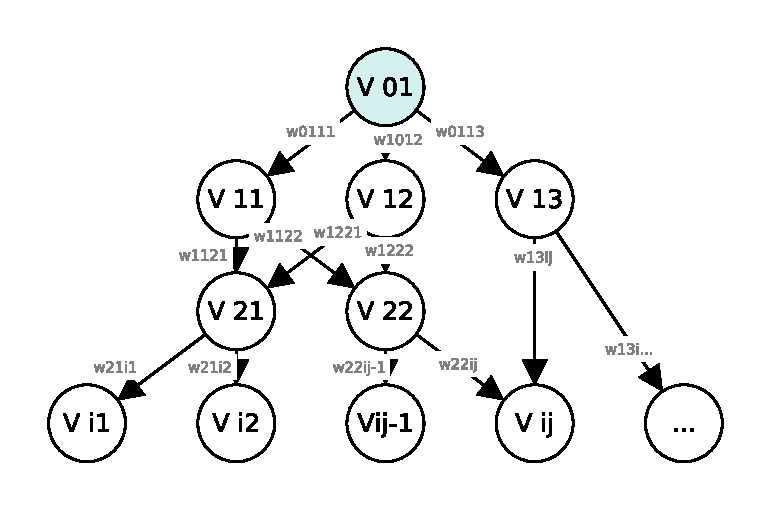
\includegraphics[width=\textwidth]{prefgraph-concept.eps}
        \caption{Shared graph}\label{fig:prefgraph-concept-shared}
    \end{subfigure}
    \begin{subfigure}{.45\linewidth}
        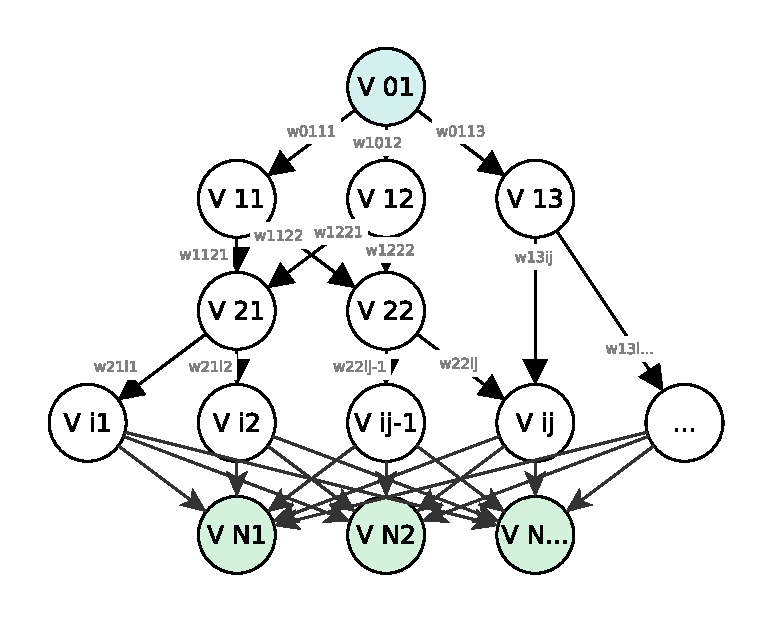
\includegraphics[width=\textwidth]{prefgraph-concept-extended.eps}
        \caption{Local graph}\label{fig:prefgraph-concept-local}
    \end{subfigure}

    \caption{\small An example of a preference graph}
    \label{fig:prefgraph-concept}
\end{figure}

However, this graph (Figure \ref{fig:prefgraph-concept-shared}) is only a part of a preference graph as it lacks
alternatives. Adding alternatives will give us the full-fledged preference graph (Figure
\ref{fig:prefgraph-concept-local}). For reasons that will soon become obvious we call the graph in Figure
\ref{fig:prefgraph-concept-shared} "shared" and the one in Figure \ref{fig:prefgraph-concept-local} "local".

With use of the weighted preference graph, a decision is made through calculating a vector of weights representing
valuability of each of the alternatives $\fnmalts$ \textit{in the context of} node $\fnmroot$ which is
achieved through iterative calculations involving intermediate nodes $\fnmnode i j$, edges, and weights.

Changing weights of any one of the preference graph's edges will change the resulting vector calculated for the alternatives
$\fnmalts$.

The following is a brief summary of our approach's key points.

\begin{itemize}
    \item The structure of neither shared nor local graphs gets changed during the simulation;
    \item Every agent may read the shared graph (Figure \ref{fig:prefgraph-concept-shared}), its weights and structure;
    \item Every agent has a predefined set of \textit{actions} assigned to it specifically;
    \item Every agent has to select an action which it will perform for a certain timespan, therefore, every action is
        mapped to the preference graph;
    \item Those alternatives, plus the shared graph form the local preference graph only visible for this agent (hence
        the name "local");
    \item Before every decision making iteration, the agent performs assessment of the alternatives $\fnmalts$ \textit{in the contexts} of
        aspects $ \fnmasps{N-1} $ using its means of local tactical assessment. Then having all the intermediate weights
        it assessess them \textit{in the context of} node $\fnmroot$. The action having the highest weight in the
        resulting vector gets selected for the execution;
    \item In parallel, some entity adjusts weights connecting the node $\fnmroot$ which we interpret as setting
        strategic objectives.
\end{itemize}

In essense we have 2 classes of entities namely a coordinator and an executor. The coordinator changes the high-most
level weights of the shared graph visible to every agent, therefore, influences decisions of the latter. At the same
time agents perform local situation assessments for their actions using their local graphs which are extensions over the
dynamically changing shared one. Changes in the shared graph get fetched and used in an individual agent's reasoning
process.

Despite the fact that necessity to adjust strategic objectives by tweaking high-level weights implies that there should be some entity that does so, we do not elaborate on its implementation.
Neither do we reveal how exactly agents' tactical reasoning processes are implemented, what are the rules of decomposing an ultimate goal that the swarm pursuits, what triggers a decision making process, and for how long an agent executes an action.
Those are details of a particular implementation which should be formulated separately with all the technical limitations, requirements, and subject area features taken into account.

% To enrich the semantics of the decomposition process, we propose to not to limit it by just one iteration.


    \section{AHP-based algorithm for fusing strategic objectives into decision making}
    \label{sect:approachFormal}

    After the generic description and the main idea of the approach have been explained, let us suggest the algorithm for
assessing the alternatives $\fnmalts$ in the context of node $\fnmroot$. And we start with laying out some definitions,
constraints, and inputs most of which are intuitive but should be stated nonetheless.

\begin{itemize}
    % TODO: context
    \item Local graph is a weighted oriented graph;
    \item It has exactly one vertex without a parent (root); it also has vertices without children (alternatives);
    \item For any 2 edges $(a,b)$, $(a,c)$, there exist no paths between $b$ and $c$ (so the local
        graph can be divided into \textit{levels});
    \item A node's \textit{level} is the maximum number of edges that should be traversed from the root $\fnmroot$ to
        achieve this node, or one of its peers;
    \item There exists a path to any alternative from any node (so we can gradually build the
        resulting vector level-by-level);
\end{itemize}

Here are notations used:

\begin{itemize}
    \item $\fnmnode i j$ denotes node $j$ of level $i$;
    \item $\fnmwasp k {\fnmnode i j}$ denotes a weights vector representing assessment of all nodes of level
        $k$ in the context of node $\fnmnode i j$;
    \item $L_i$ denotes an index set for nodes of level $i$.
\end{itemize}

As an input, we have a preference graph (local graph) $\left< V, E, W \right>$ ($V$ - nodes, $E$ - edges, $W$ - weights)
having $N$ levels (it is assumed that $N>2$, otherwise the problem is trivial).
Weights for intermediate levels and the root are predefined, i.e. we have a set
$\fnmsetind
    {\fnmwasp{l}{\fnmnode{l-1}{i}}}
    {i \in L_{l-1}, l = \fnmrange{1}{N-1}}
$.

In the result, it is required to calculate $\fnmwasp N \fnmroot$ vector representing weights for actions adjusted for
strategic preferences, and assign an agent with whatever action has the maximum weight assigned to it. To achieve that, we
propose to use \textit{AHP} \cite{saaty-2008} algorithm which enables one to assess alternatives using preference
weights of 2 intermediate levels:
%TODO: AHP, reference

\begin{equation}
    \fnmwasp a {\fnmnode {a-2} x} =
    \fnmAhp
        {\fnmSetWasp{a}{a-1}}
        {\fnmwasp {a-1} {\fnmnode {a-2} x}}.
\end{equation}

This property of the \textit{AHP} algorithm means that once lower-level weights (tactical assessment) have been
estimated, we can calculate vector $\fnmwasp N \fnmroot$ by iteratively assessing the alternatives in contexts of
vertices of levels $N-2$, $N-3$, and so on up to the root $\fnmroot$. It is possible since every alternative is
reachable from any node, so we can assess alternatives in any context. So, when strategic reasoning, iterative weights
assessment, and action selection based on this assessment are put together, the resulting algorithm for an agent will
look as shown in Listing \ref{lst:agent-reason}

\begin{algorithm}[h!]
    \floatname{algorithm}{Listing}
    \caption{Agent's reasoning process}
    \label{lst:agent-reason}

    \begin{algorithmic}[1]
        \State {\textbf{Input:} $\fnmsetind {\fnmwasp{l}{\fnmnode{l-1}{i}}} {i \in L_{l-1}, l = \fnmrange{1}{N-1}} $}
        \State {\textbf{Input:} \textbf{procedure} \fnlCall{AHP}{2}}
        \State {\textbf{Input:} \textbf{procedure} \fnlCall{assessTactical}{}}
        \State {\textbf{Input:} \textbf{procedure} \fnlCall{perform}{1}}
        \State {\textbf{Input:} $\left< V, E, W \right>$ local graph}

        \\

        \Procedure{assess}{$\fnmSetWasp{N}{k}$, k}

        \\ \Comment{The root node has been reached}

            \If{k = 1}
                \State {\textbf{return} \fnlCall{AHP}{$\fnmSetWasp{N}{k}$, $\fnmwasp{1}{\fnmroot}$}}

                \\ \Comment{Assessing the alternatives $N$ in}
                \\ \Comment{higher-level contexts (decreasing $k$)}
            \Else
                \State {\textbf{return} \fnlCall{assess}{$\big\{ \fnlCall{AHP}{\fnmSetWasp{N}{k}, \fnmwasp{k}{\fnmnode{k-1}{i}}} \big\}_{i \in L_{k-1} }$, k-1}}
            \EndIf
        \EndProcedure

        \\

        \Procedure{run}{}
            \While{simulationContinues}
                \State{ $\fnmSetWasp{N}{N-1} \gets \fnlCall{assessTactical}{}$ }
                \State{ $W \gets W \cup \fnmSetWasp{N}{N-1}$ }
                \State{ weights $\gets \fnlCall{assess}{\big\{ \fnlCall{AHP}{\fnmSetWasp{N}{N-1}, \fnmwasp{N-1}{\fnmnode{N-2}{i}}} \big\}_{i \in L_{N-2} }$, N-2}}
                \\ \Comment{weights = $(w_1,w_2,...)$}
                \State{action $\gets \arg_{w_i} \max$ weights}
                \State{\fnlCall{perform}{action}}
            \EndWhile
        \EndProcedure

    \end{algorithmic}
\end{algorithm}



    \section{"Relay race" load balancing algorithm}

intro


In \cite{murashov-2022}, an agent would receive an input comprising preference hierarchy graph with pre-defined weights, the task itself, and meta-information regarding required technical capabilities a runner must possess.
Then it would compare its own state with that of its neighbours, assess those in the context of criterion used by the cluster, and make a pass-or-keep decision.
The set of those criterion consists of performance metric, energy efficiency, and load distribution uniformity.

Since the goal here is to achieve separation of local and global decision making, this preference hierarchy must be extended by additional levels.


\begin{figure}[hbt!]
    \centering
    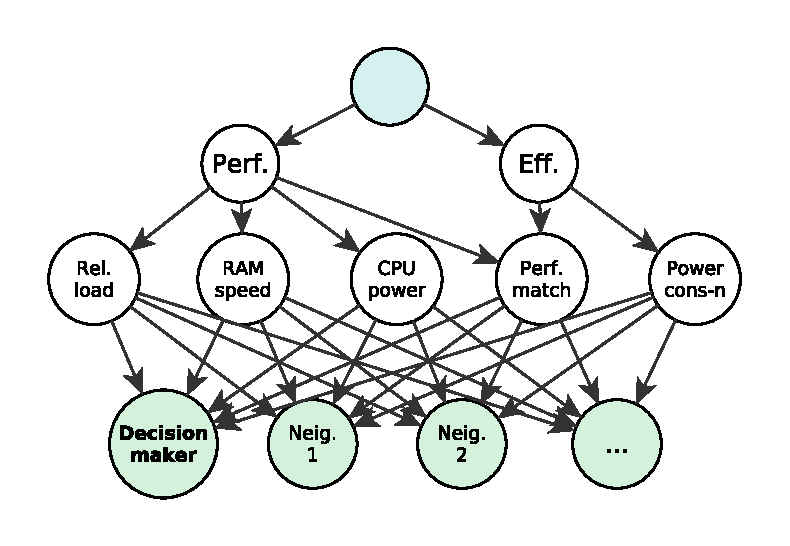
\includegraphics[width=.8\textwidth]{prefgraphLb.eps}
    \caption{Preference hierarchy for load balancing}
    \label{fig:prefgraphLb}
\end{figure}


Once an agent has received "high-level" weights, it must update its local preference hierarchy graph.
After that it should update the list of its neighbours, assess them against lower-level criterion (while taking features of the task to be assigned into consideration), and make the decision on whether to pass the task to some other node, or run it now.

% TODO ref. listing
This reasoning process is equivalent to that described in listing \ref{lst:agent-reason}, only a bit detailed.
In the case we describe, the "perform" procedure consists of either running the task, if the selected node number is equivalent to that of the decision making node, or pass it to the best matching neighbour.

% TODO ref. listing
We will not elaborate on how exactly assessments in the context of a criteria can be done (procedure "assess" in listing \ref{lst:agent-reason}), because this topic is complicated enough to be a research of its own.
But probably the best (the most practical) way to do so is to devise a set of heuristic measures.
Success of the aforementioned "Kubernetes" which uses engineeric heuristics suggests that the lack of solid theoretical foundations in this particular aspect will not be too much of an impediment.

% TODO: ref listing
Asynchronously with network nodes, a coordinator performs the following set of operations. It monitors the network state and infers weights for higher levels of the preference hierarchy. Occasionally, it receives a task and passes it to any node (which may remain the same every time).


    \label{sect:relayRace}

    \section{Conclusions}

The next generation of networks require formal foundations they reside upon to be able to handle high volatility of a network's topology.
Thus centralized control systems become more and more obsolete.
So we are glad to propose a solution that strikes the right balance between the necessity to control a system, the flexibility, and simplicity.

By this paper, we propose a new approach to solving load balancing problem through use of a combination of "relay race" and AHP algorithms.
The latter enables separation of strategic and tactic reasoning thus allowing the best-fit solutions to emerge, while the former, being indifferent to the topology of a system, takes care of its volatility aspect.
We also developed two extensible algorithm for both individual agents of a system (network nodes), and the coordinating entity that monitors the state of a network.


Here are the directions of this work's further development we would like to suggest.
The first one is creating an ontology of load balancing quality measures (or searching for an existing one that fits the purpose).
As we have stated before, the preference hierarchy we have proposed before (Figure \ref{fig:prefgraphLb}) only serves the immediate purpose of being an illustrative example.
Creating such an ontology would, in turn, enable creating a more generalized preference hierarchy graph.

Once an ontology is defined, finding good quality measures becomes the next step.
Our previous work \cite{murashov-2022} might serve as a starting point in this endeavour.
Some of measures used there might highlight some good solutions, on conceptual level at least.

An experiment.
Although what has been proposed here is an observable iteration over \cite{murashov-2022} which offers proven results of a simulation that tests our core ideas, substantial and provable results of an experiment for this particular work are still required.


    \label{sect:conclusion}

    This research is partially supported by the Russian foundation for basic research (grant № FFZF–2022–0004).


    \medskip

    \bibliographystyle{splncs04}

    \bibliography{bib}

\end{document}
